\subsection{Themapagina}\label{themapagina}

Hieronder volgt een beschrijving voor het aanmaken van een themapagina.

\begin{center}
	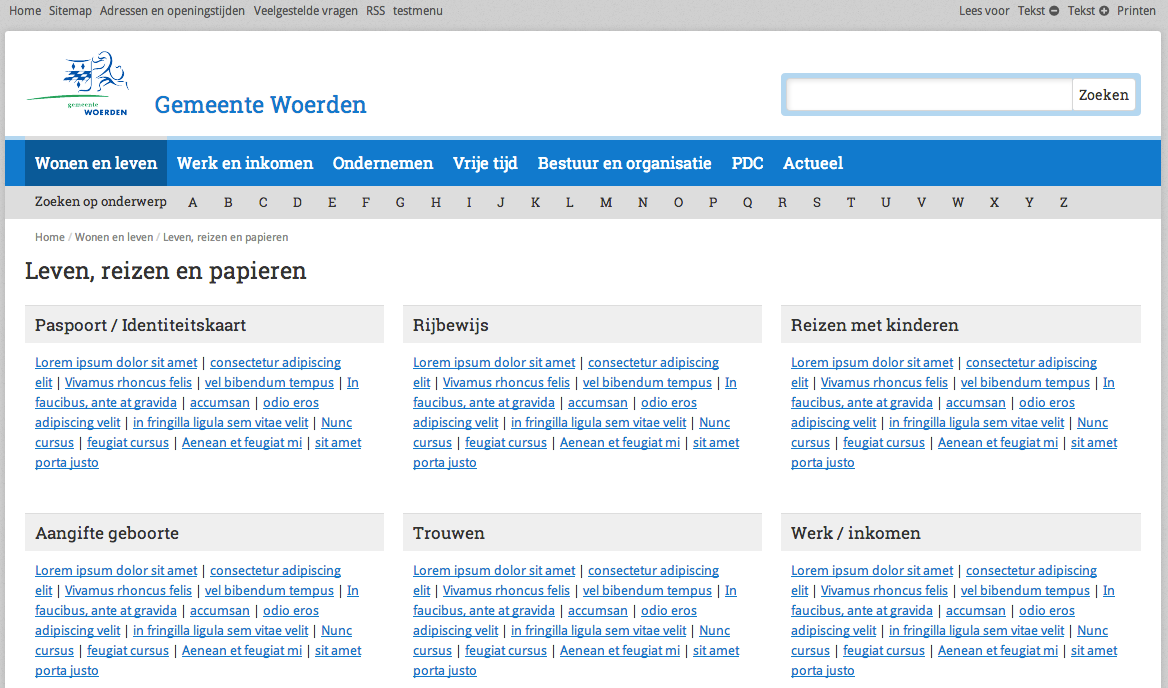
\includegraphics[width=\textwidth]{img/themapagina.png}
\end{center}

\begin{enumerate}
\item Ga naar node/add/subject en maakt een nieuw \emph{Onderwerp}\seeone{onderwerp} aan. In dit voorbeeld maken we het onderwerp \emph{Afval} aan onder het menuitem \emph{Wonen en leven}.
\item Vul als titel \emph{Afval} in.
\item Laat de body leeg (optioneel).
\item Scroll naar onderen en selecteer "URL-pad-instellingen\emph{, vink het vinkje uit en vul }wonen-en-leven/afval" als URL.
\item Sla het item op.
\item Bewerk het hoofdmenu (admin/structure/menu/manage/main-menu).
\item Bewerk het menuitem \emph{Afval} en vul bij pad "wonen-en-leven/afval" in.
\item Navigeer via het menu naar de zojuist aangemaakt pagina, wonen-en-leven/afval. Deze pagina kan nu gevuld gaan worden met \emph{Felix}\seeone{felix} blokken.
\item Ga naar node/add/editorial en maakt een nieuw item aan. Dit is het item wat we gaan gebruiken als blok op de themapagina. De titel en body zijn vrij in te vullen.
\item Ga naar wonen-en-leven/afval en voeg een blok toe aan een van de regio's: Regio 4/12 first, Regio 4/12 second of Regio 4/12 third.
\item Kies daarbij uit nodetype \emph{Editorial}, daarna \emph{Volledige inhoud} en selecteer het zojuist aangemaakte item.
\item Na opslaan zal het blok zichtbaar zijn op de pagina. Herhaal de stappen 9 /tm 11 om meerdere blokken toe te voegen aan de pagina.
\end{enumerate}